\subsection{Aims and Scope}

Begin with introducing the problem and reasoning behind team's interest in building a dashboard in context of this problem. 

This section will summarize the objectives this dashboard aims to achieve. 

\subsubsection{Topic and targeted policymaker.}
Describe the main topic and policymaker you selected here

\paragraph{Context}
~\\ PLACEHOLDER: Netherlands Housing Market, American Housing Market, Changes in Housing Prices since 1950 etc. 

% \paragraph{Data included in the analysis:} 
% ~\\ Population in each street-level pincode in the Netherlands, Number of hospitals in each city, etc.

\subsubsection{Targeted stakeholders and identified information needs.}
Describe the stakeholders at the policymaker or business leadership level and their information needs.  

\subsubsection{Key Performance Indicators and Critical Success Factors}
Describe the KPIs and CSFs here aligned with the targeted stakeholders/information needs. The KPIs and CSFs need to be measurable and identifiable for the stakeholders such that it is actionable for a policymaker when being presented to them.

An example: 
\begin{table}[h]
\centering
\caption{CSF-to-KPI Mapping for Dashboard Design}
\begin{tabularx}{\textwidth}{l X X l}
\toprule
\textbf{CSF} & \textbf{KPI} & \textbf{Chart Type} & \textbf{Data Source}\\
\midrule
Customer retention & Monthly churn rate & Line chart (trend) & CRM export \\
Customer retention & Customer lifetime value & Bar chart by segment & Billing system \\
Customer retention & Repeat purchase rate & Line chart (trend) & Order database \\
\bottomrule
\end{tabularx}
\end{table}

\subsubsection{Our contribution.}
What you contribute \& how it creates value

\subsection{Related Projects and Dashboards}
In the first phase of the project, you must have gone through several publicly available dashboards and those mentioned in academic research. You can also search for similar projects in enterprise level that may have been mentioned in the media. Why are these dashboards good at what they do, why could they be useful for you, what could be improved and which gap remains after all the related projects. The following example highlights examples built in past few years to study the spread of Covid-19. 

The two most related dashboards to ours are the Confirmed Infections Dashboard by RIVM\footnote{\url{https://coronadashboard.government.nl}, retrieved \today.}, shown in Fig.~\ref{fig:reldashboards:1}, and the Confirmed Infections Dashboard by RIVM\footnote{\url{https://coronadashboard.government.nl}, retrieved \today.}, shown in Fig.~\ref{fig:reldashboards:2}. \todo{Replace by the 1-3 most related dashboards you found on the web.}

\begin{figure}[h!]
  \centering
  \begin{subfigure}{.49\textwidth}
    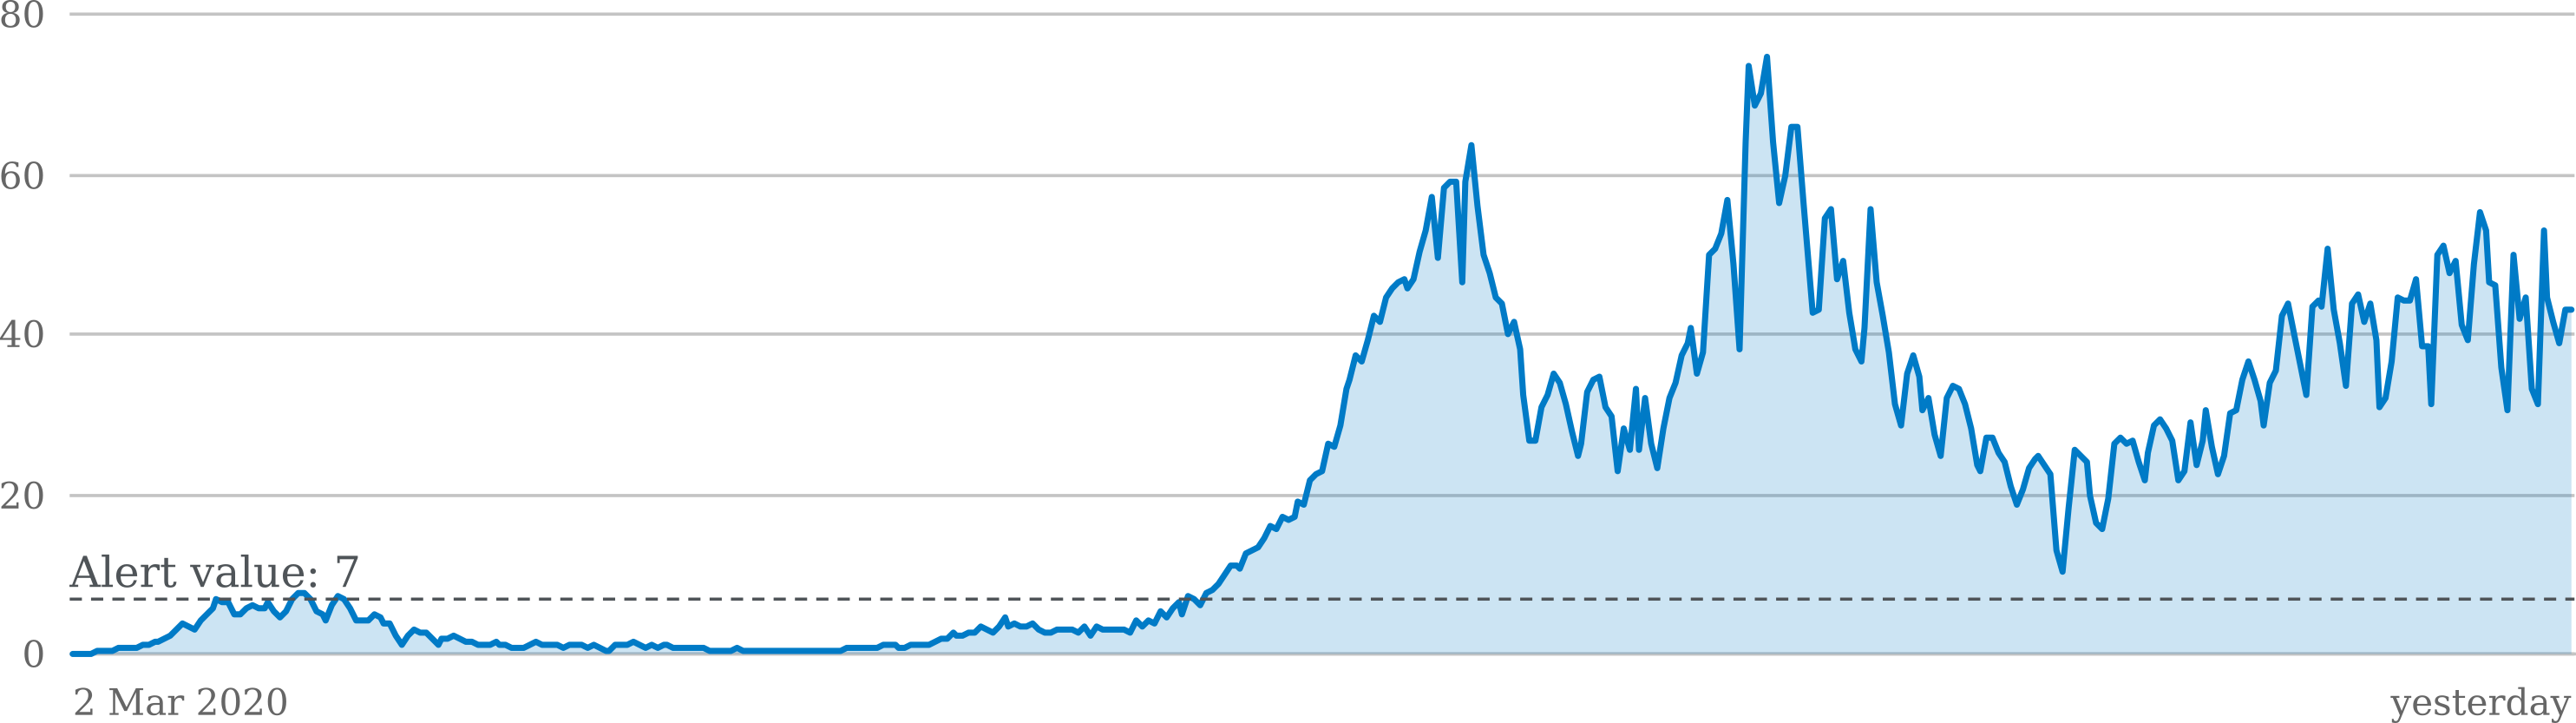
\includegraphics[width=\textwidth]{fig/infections_2021_may.png}
    \caption{RIVM Confirmed Infections}
    \label{fig:reldashboards:1}
  \end{subfigure}
  \begin{subfigure}{.49\textwidth}
    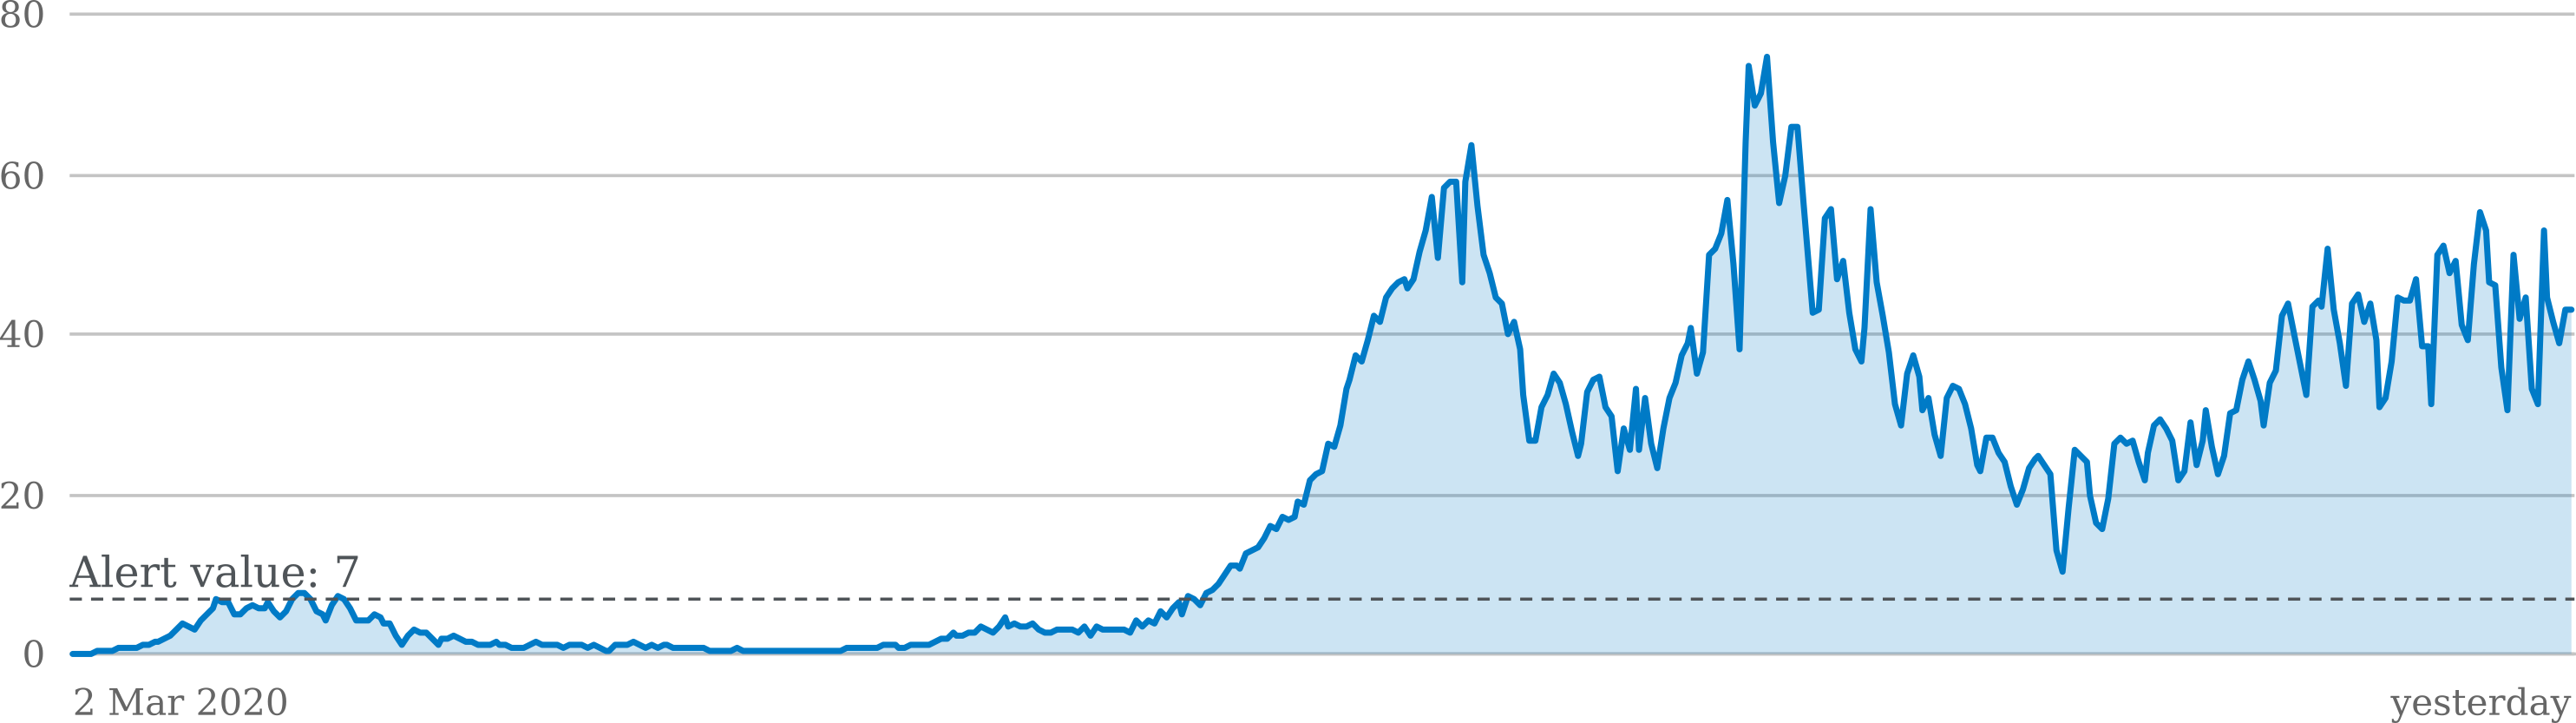
\includegraphics[width=\textwidth]{fig/infections_2021_may.png}
    \caption{RIVM Confirmed Infections}
    \label{fig:reldashboards:2}
  \end{subfigure}
  \caption{The most related dashboards.}
\end{figure}

\paragraph{RIVM Dashboard.}
Replace with your description

\paragraph{The other RIVM Dashboard.}
\footnote{\url{https://coronadashboard.government.nl}, retrieved \today.}
Replace with your description


\subsection{Summary of our Approach.}
Here, we provide a brief summary of our approach\todo{Edit: Summarise the \textbf{how} of your implementation}, before summarising the data sources, the analytics and visualisations, and the evaluation and deployment below. A mock-up / screenshot of our interactive dashboard is given in Fig.~\ref{fig:ourdashboard:1}-\ref{fig:ourdashboard:2}.

It is possible that your approach will change over time as you begin to explore more data sources and learn various methods in this course. This section would highlight your current plans. \\

For the \textbf{concept report}: This should entail your current plan on how to go about the data, visualisations and evaluation \& deployment just as written down here in the headers \\

For the \textbf{final submission}: This should entail an introduction on your methodology and data for the final part. Data Sources should be fully done in the data dictionary which is added as a seperate document, where here you just have to summarise the data that is used in the project. The analytics and visualisations should logically be in chapter 2, where here you just introduce it. The evaluation and deployment should logically be in chapter 3, where here you just introduce it. The headers below may be removed from Chapter 1, since they will be found elsewhere in the document. \\

\subsubsection{Data sources.}
Summarise the data sources and their integration, before they are described one-by-one. Note: The question ‘What is the format of the data?’ will be analysed in more detail under the Data Preparation and Modelling section which falls out of scope for the Concept Report. In this section, simply state the format (file type) and update frequency.
\todo[inline]{Enter a description for all your data sources here, including their relevance to the KPI. A good starting point for data sources on the Netherlands is: \url{https://data.rivm.nl/covid-19/}. When describing the data sources, please include the link to the data source.}
% \paragraph{Netherlands: RIVM COVID-19 Casus Landelijk}
% \begin{description}
%   \setlength\itemsep{0em}
%   \item[Scope:] Netherlands, daily infections cases with demographics and outcomes
%   \item[Source:] RIVM \url{https://data.rivm.nl/covid-19/COVID-19_casus_landelijk.html}
%   \item[License:] Open access, Public Domain Mark 1.0
%   \item[Format:] CSV, updated daily at 15:15
%   \item[Import:] Daily ETL
%   \item[Known issues:] Change (relaxation) of testing requirements on 2020-06-01.
% \end{description}

\subsubsection{Analytics and visualisation.}
“Describe which analytics and visualisations will be implemented, what information they will present, and which of them will be interactive.”
\begin{figure}[h]
  \centering
  \begin{subfigure}{.49\textwidth}
    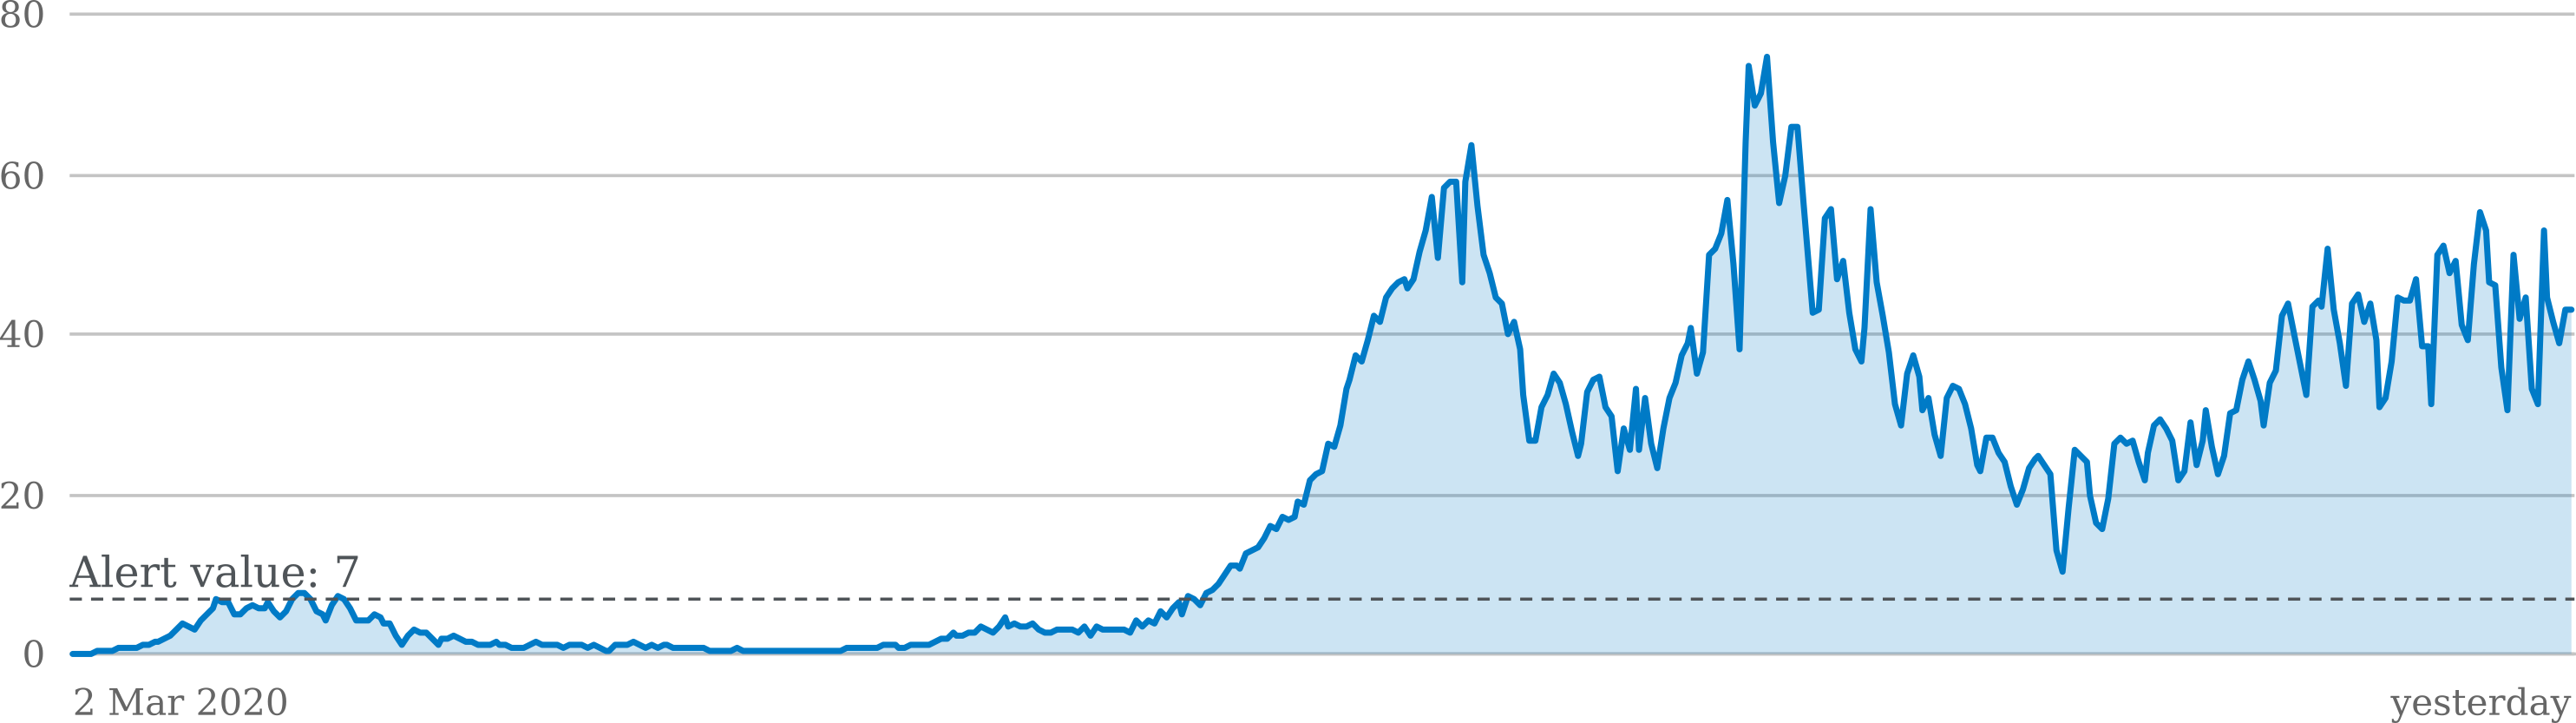
\includegraphics[width=\textwidth]{fig/infections_2021_may.png}
    \caption{View 1}
    \label{fig:ourdashboard:1}
  \end{subfigure}
  \begin{subfigure}{.49\textwidth}
    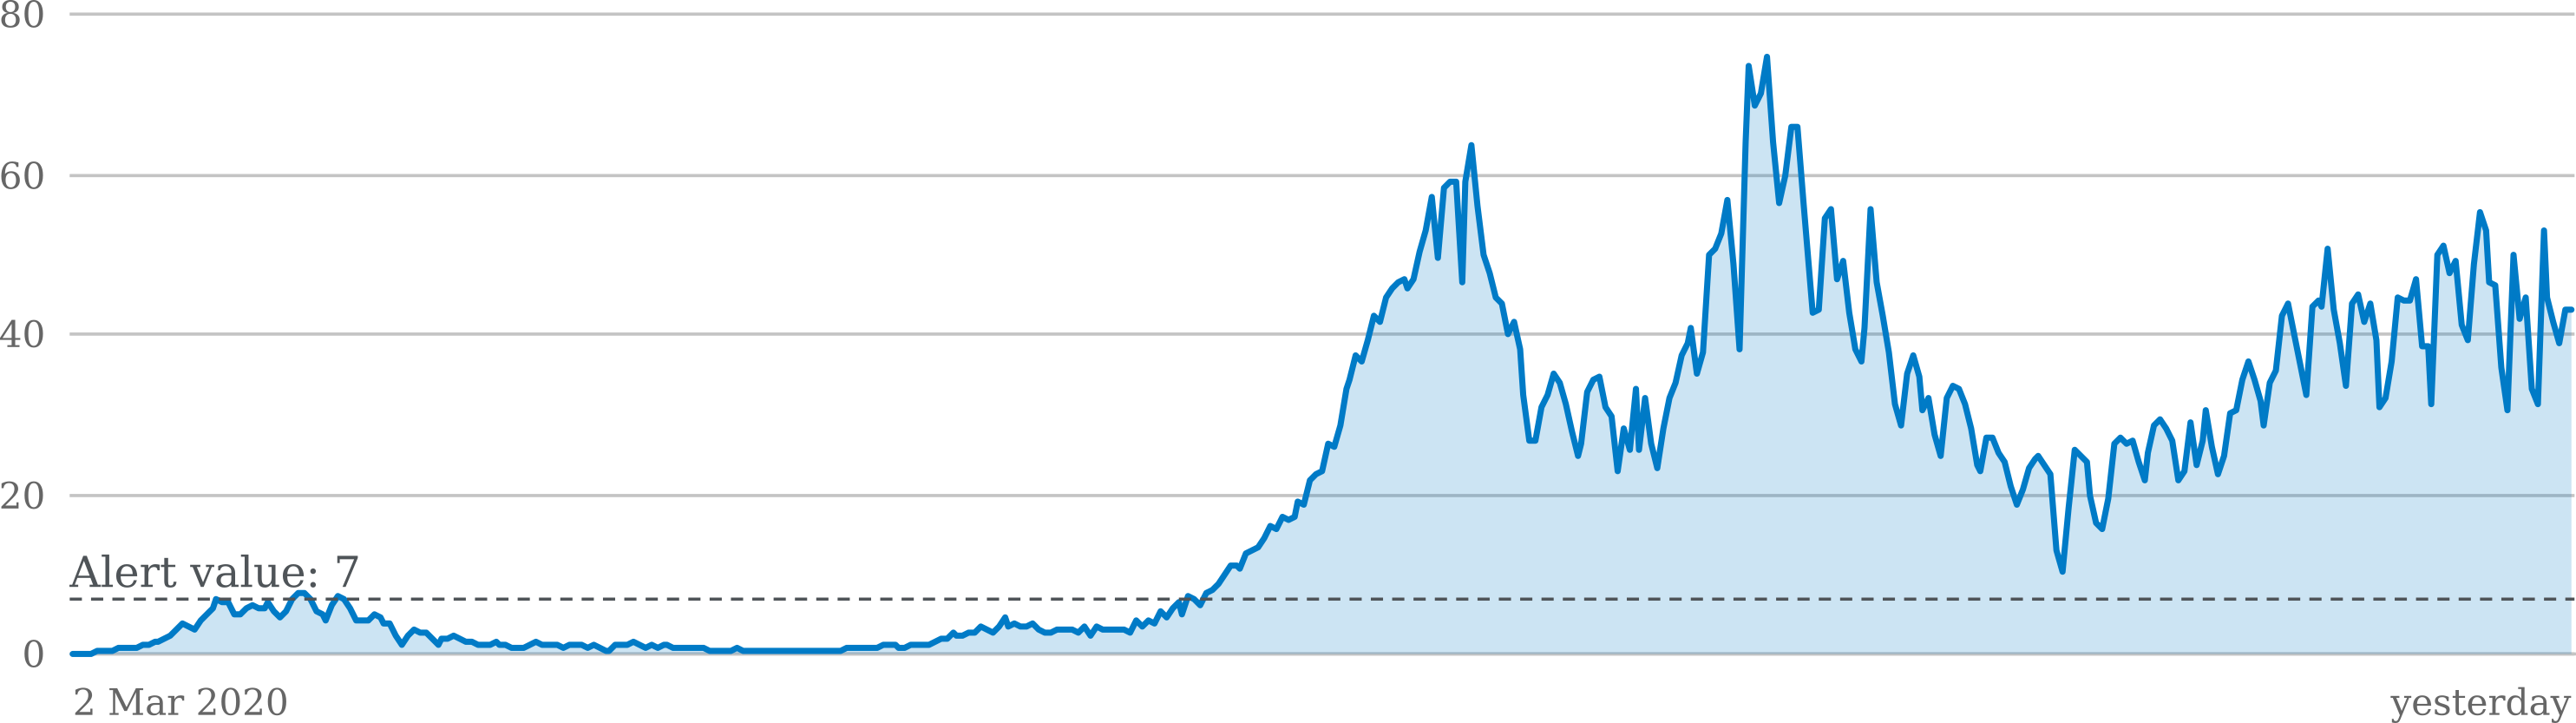
\includegraphics[width=\textwidth]{fig/infections_2021_may.png}
    \caption{View 2}
    \label{fig:ourdashboard:2}
  \end{subfigure}
  \caption{Mock-up of our dashboard.}
\end{figure}

\subsection{Planned Evaluation and Deployment.}

\subsubsection{Criteria of success and evaluation.}
Criteria, evaluation plan
I.e. when is the dashboard succesful for a stakeholder? When is it good for the policymaker? What are shortcomings and future plans for the dashboard etc. This list is not exhaustive, just an example. Please add onto it what the team finds necessary. 

\subsubsection{Deployment and maintenance.}
Needs for deployment \& maintenance 
An example: \url{https://medium.com/@amarakoonanjalee11/understanding-sdlc-deployment-maintenance-the-final-phase-d2a6b26cf9e0} 
\\
\textbf{Do not make any assumptions! I.e. an uptime of 99\% should be motivated why it is necessary. An uptime of 99\% as-is is not feasible if the computing power required is a lot or when the dashboard is only used once-twice a month. If you do not know the situation at the policymaker, tell us how they can make this dashboard succesful, deployable and maintainable for the future.} \\ \\
At this point the concept report stops and has reached a maximum of 4 pages excluding the front page, contents and  Appendix. Do not include the hours logged.

